\section{Introduction}
%% Chapter 3: functional diversity analyses
%Dormann 2012 Collinearity: a review of methods to deal with it and a simulation study evaluating their performance
% Mouillot et al 2014 
\section{Methods}

\subsection{Data sources and trait selection}

\subsubsection{The PREDICTS database: using a `space for time' substitution to assess the impacts of land-use change on local vertebrate communities.}
The impacts of land-use change on the functional diversity of vertebrate communities was assessed using a `space for time' substitution. A longitudinal approach would require data on the evolution of local community composition as the landscape changes from pristine to disturbed, with experimental designs such as `before-after-control-impact' (REF). Nevertheless, such data is difficult to obtain at large scales for diverse taxa and for multiple types of environmental change. With the space for time substitution, a spatial gradient is used as a proxy for temporal dynamics. This approach facilitates meta-analytic studies, as data on the community composition of local assemblages in various land-uses is both easier to collect and more abundant. 

Such data was compiled in the PREDICTS database (ref). This database is, to my knowledge, the most comprehensive global collection of studies that sampled biodiversity across diverse land-uses. In all studies, species abundance (in most cases) or occurrence was recorded across a variety of sites, each characterised by a land-use. Land-use was divided into six categories: primary vegetation, secondary vegetation, plantation forest, cropland, pasture and urban. Secondary vegetation was further divided in three categories (mature, intermediate and young) according to the stage of recovery of the vegetation. %This global database as such allows to conduct meta-analytic studies of the impact of land-use change on terrestrial communities, using a space for time substitution.

I sub-setted the PREDICTS database to retrieve all the sites where vertebrate species were sampled. I selected studies for which the same set of species was consistently sampled across sites, and for which more than one species was considered. Overall, 180 studies were selected (total of 6758 sites). Of these, abundance data was available for 132 studies, and occurrence data for the remaining 48 studies. Figure \ref{PREDICTS_maps} shows the location of all the sites that were considered.

\begin{figure}[h!]
\centering
\includegraphics[scale=0.75]{figures/chapter3/Sites}
\caption[Location of selected PREDICTS sites]{\textbf{Location of selected PREDICTS sites.} 180 studies containing occurrence or abundance data for terrestrial vertebrates were selected in the PREDICTS database. Of these, 132 studies provided species relative abundance (corresponding sites are shown in blue on the map). An additional 48 studies only recorded species presence--absence (corresponding sites shown in red).}
\label{PREDICTS_maps}
\end{figure}

As the PREDICTS database was built by collating data from independent studies, its design was imbalanced by construction. As such, nearly half of the selected studies only sampled birds, and nearly 80\% of the studies considered one class only (Table \ref{class_compo}). About 17\% of the studies sampled species from different classes. 

\begin{table}[!htbp] 
\renewcommand{\baselinestretch}{1}
\renewcommand{\arraystretch}{1.2}
\begin{center}\fontsize{9}{11}\selectfont
  \caption[Vertebrate classes considered in selected studies]{\textbf{Vertebrate classes considered in selected studies.} As the PREDICTS database consists of a collation of independent studies...} 
  \label{class_compo} 
\begin{tabular}{@{\extracolsep{1pt}} lcc} 
\\[-1ex]\hline 
\hline \\[-1ex] 
\textbf{Class} & \textbf{Number of studies} & \textbf{\% studies} \\ 
\hline \\[-1ex] 
Birds & $87$ & $48.3$ \\ 
Mammals & $37$ & $20.6$ \\ 
Amphibians & $18$ & $10$ \\ 
Amphibians, Reptiles & $10$ & $5.6$ \\ 
Birds, Mammals & $9$ & $5$ \\ 
Reptiles & $8$ & $4.4$ \\ 
Amphibians, Mammals, Reptiles & $5$ & $2.8$ \\ 
Amphibians, Birds, Mammals, Reptiles & $2$ & $1.1$ \\ 
Birds, Mammals, Reptiles & $2$ & $1.1$ \\ 
Mammals, Reptiles & $2$ & $1.1$ \\ 
\hline \\[-1.8ex] 
\end{tabular} 
\end{center}
\end{table} 

Similarly, the number of sites sampled in each land-use category differed across studies. Table \ref{sample_size_LU} shows the sample size (number of sites) for each land-use category (based on all 180 studies). 

\begin{table}[!htbp]
\renewcommand{\baselinestretch}{1}
\renewcommand{\arraystretch}{1.2}
\begin{center}\fontsize{9}{11}\selectfont
  \caption[Sample size for each land-use category]{\textbf{Sample size for each land-use category.} The number of sites in each land-use is reported here across 180 selected studies.} 
  \label{sample_size_LU} 
\begin{tabular}{@{\extracolsep{5pt}} lcc} 
\\[-1.8ex]\hline 
\hline \\[-1.8ex] 
\textbf{Land-use} & \textbf{Number of sites} & \textbf{\% sites} \\ 
\hline \\[-1.8ex] 
Primary vegetation & $2,569$ & $38.0$ \\ 
Plantation forest & $1,151$ & $17.0$ \\ 
Cropland & $888$ & $13.1$ \\ 
Pasture & $808$ & $12.0$ \\ 
Young secondary vegetation & $501$ & $7.4$ \\ 
Intermediate secondary vegetation & $350$ & $5.2$ \\ 
Urban & $292$ & $4.3$ \\ 
Mature secondary vegetation & $199$ & $2.9$ \\ 
\hline \\[-1.8ex] 
\end{tabular} 
\end{center}
\end{table} 


\paragraph{Trait selection for the calculation of functional indices.}
In Chapter 3, I collected and imputed the values of ten traits across terrestrial vertebrates. Trait data was used in the current Chapter to calculate functional diversity indices. A crucial step was to select the traits to include in the calculations. Indeed, functional diversity indices can be sensitive to the number of traits (Mouillot et al 2014). On the one hand, not including enough traits may lead to missing important areas in the multidimensional trait space. On the other hand, when there is multicollinearity among the traits, functional indices may be inflated. Multicollinearity can create a form of redundancy in the multidimensional trait space, problematic for the calculation of the indices. Assessing whether traits were linearly related to each other was as such a necessary step. 

I randomly selected one imputed trait dataset among the eight imputed datasets (see Chapter 1). To improve normality, a log-10 transformation was applied to all continuous traits (except habitat breadth, which was square-rooted). Trait values were also centred and scaled to zero-mean and unit-variance across the four vertebrate classes. All traits were subsequently considered, except those relating to species diet (primary diet and diet breadth), as these were unavailable for reptiles. As such,the traits taken into consideration were: body mass; longevity; litter/clutch size; habitat breadth; habitat specialisation; diel activity; trophic level.

\begin{comment}
\subparagraph{Dimensionality reduction}

%To first assess if collinearity could be a problem, I used a clustering approach for mixed-type data (factor analysis of mixed type data, or FAMD, ref) to represent the contribution of each variables to principal components. The graph shows that body mass - longevity might e correlated and that BM-LCS could be negatively correlated.


\begin{figure}[h!]
\centering
\includegraphics[scale=0.75]{figures/chapter3/Graph_traits_variables}
\caption[]{\textbf{}}
\label{}
\end{figure}

\begin{figure}[h!]
\centering
\includegraphics[scale=0.75]{figures/chapter3/Individual_factor_map}
\caption[]{\textbf{}}
\label{}
\end{figure}

\begin{figure}[h!]
\centering
\includegraphics[scale=0.75]{figures/chapter3/Quantitative_variables}
\caption[]{\textbf{}}
\label{}
\end{figure}
\end{comment}

\subparagraph{Assessing the degree of multicollinearity across traits.}
To first assess whether multicollinearity could be a problem, I estimated Pearson's pairwise correlation coefficients among continuous traits, as high correlation coefficients can be an indicator of collinearity. A threshold of 0.7 is usually used for detecting potential collinearity (Dormann 2012). The determinant of the correlation matrix can also be assessed, with values close to 0 indicating high degrees of multicollinearity (Dormann 2012).

Table \ref{corcont} shows the pairwise correlation coefficients among continuous traits. Body mass and longevity were the two variables that had the highest correlation coefficient (0.51). The determinant of the correlation matrix was 0.67, thus indicating that the degree of multicollinearity was likely to be low among continuous traits. 

\begin{table}[!htbp] \centering 
\renewcommand{\baselinestretch}{1}
\renewcommand{\arraystretch}{1.2}
\begin{center}\fontsize{9}{11}\selectfont
  \caption{} 
  \label{corcont} 
\begin{tabular}{@{\extracolsep{5pt}} lcccc} 
\\[-1.8ex]\hline 
\hline \\[-1.8ex] 
 & Body mass & Longevity & Litter/clutch size & Habitat breadth \\ 
\hline \\[-1.8ex] 
Body mass & $1$ & $$ & $$ & $$ \\ 
Longevity & $0.509$ & $1$ & $$ & $$ \\ 
Litter/clutch size & $$-$0.146$ & $$-$0.083$ & $1$ & $$ \\ 
Habitat breadth & $0.167$ & $0.134$ & $0.194$ & $1$ \\ 
\hline \\[-1.8ex] 
\end{tabular} 
\end{center}
\end{table}

Nevertheless, the previous diagnostics did not take into consideration categorical traits. Potential associations between categorical and continuous traits, or among categorical traits, also needed to be assessed. To that end, I used generalised variance inflation factors (GVIF) or variance inflation factors (VIF), as developed by Fox and Monette (1992), to detect multicollinearity across all traits. Given a regression model, variance inflation factors quantify the overestimation in the variance of estimated regression coefficients due to multicollinearity among the predictors. A VIF or GVIF value of 5 or 10 is commonly used as a threshold to select out collinear predictors (Dormann 2012). I used the function stepwise.vif of the package Rnalytica (ref), in which a normally-distributed dummy variable was used as a dependent variable in a linear regression model where all traits were used as predictors. The VIF or GVIF of each predictor was then assessed.  Multicollinearity across predictors was not detected to be problematically high, as all predictors had a VIF or GVIF value below 2 (Table \ref{GVIF}). As such, all the traits figuring in Table \ref{GVIF} were included in the calculations of functional indices. 

% https://www.rdocumentation.org/packages/pedometrics/versions/0.6-6/topics/stepVIF
%% Table GVIF values among traits
\begin{table}[!h]
\renewcommand{\baselinestretch}{1}
\renewcommand{\arraystretch}{1.2}
\begin{center}\fontsize{9}{11}\selectfont
  \caption[Variance inflation factor of estimated regression coefficient for each trait treated as a predictor in a linear regression model.]{\textbf{Variance inflation factor of estimated regression coefficient for each trait treated as a predictor in a linear regression model.} For categorical traits, the GVIF was calculated rather than the VIF. All traits had a VIF or GVIF below 2: multicollinearity was not problematic among the traits.} 
  \label{GVIF} 
\begin{tabular}{@{\extracolsep{5pt}} lc} 
\\[-1ex]\hline 
%\hline \\[-1.8ex] 
 Predictor & VIF or GVIF \\ 
\hline \\[-1.8ex] 
Diel activity & $1.145$ \\ 
Litter/clutch size & $1.267$ \\ 
Trophic level & $1.288$ \\ 
Specialisation & $1.391$ \\ 
Longevity & $1.441$ \\ 
Habitat breadth & $1.473$ \\ 
Body mass & $1.584$ \\ 
\hline \\[-1.8ex] 
\end{tabular} 
\end{center}
\end{table} 


\subparagraph{Ecological relevance of the traits.} See Introduction to Chapter 3. 
% body mass; longevity; litter/clutch size; trophic level;  habitat breadth; degree of habitat specialisation; and diel activity.

\subsection{Definition and calculation of functional diversity indices}


\subsubsection{Calculation of functional diversity metrics across PREDICTS vertebrate communities}
Functional diversity indices were calculated for each local vertebrate community of the PREDICTS database (in other words, for each PREDICTS site, Figure  \ref{FDcalc_chart} A). All indices were calculated across the 180 studies for which species occurrence was available. In addition, indices which could be abundance-weighted were calculated across the 132 studies which provided species relative abundance. 

Rao's quadratic entropy was calculated using the dbFD package (ref).

\subsection{Assessing the impacts of land-use change on functional diversity indices}

	\subsubsection{Functional indices independent from species richness}

	\subsubsection{Functional indices dependent on species richness}

		\paragraph{How does land-use change impact the species-richness--functional richness relationship?}

		\paragraph{Disentangling the effects of species richness from the effects of land-use on functional diversity indices through simulations: an adequate approach with PREDICTS?}

\subparagraph{Approach.}
Functional diversity metrics, notably those aiming at estimating functional richness, can be correlated with species richness. For such indices, disentangling the effects of species richness from the effects of land-use is vital. Indeed, an observed decrease in the main effect of land-use on a functional richness index correlated with species richness may be driven by changes in species richness alone. Above, I detailed how investigating how land-use change affects the species richness -- functional index relationship allows to overcome the species richness problem. Here, I focus on an alternative approach to disentangle the effects of species richness from the effects of another environmental variable.

This approach is based on the randomisation of the species composition of local assemblages. Given a species richness, randomising community composition \textit{m} times allows to generate null expectations of the values of functional indices. These null expectations can then be compared to the empirical (observed) values. Along a species richness gradient, such an approach allows to understand the impact of the variable of interest independently from the impact of species richness on the calculated metrics. Here, such an approach was not necessary \textit{per se}, as most indices were independent from species richness by construction, and for those that were not, I focused on the relationship between species richness and the index rather than on the mean effect of land-use on the effect. Nevertheless, I implemented a simulation approach aiming at examining whether it would be a suitable method given the PREDICTS database.

Specifically, the community composition in each site was randomised by re-sampling species in the corresponding study's species pool, maintaining the species richness of each site (Figure \ref{FDcalc_chart}). Community composition was randomised 1000 times (for metrics calculated with dbFD) or 10,000 times (for DFR). For each randomised community in each site, the functional diversity indices were calculated. Null expectations of functional diversity indices were then generated for each site by taking the median value obtained across simulations.

Although only DFR was strongly correlated with species richness, I implemented this simulation approach for all functional indices that I considered. My expectations were that:
\begin{itemize}
\item For indices independent from species richness by construction, the mean effect of land-use on simulated indices should be similar. Specifically, the mean effect observed for primary vegetation, the most pristine land-use type in the dataset, should not differ from the mean effect observed in other land-uses (\textit{expectation 1}).
\item For indices that correlate with species richness, the slope of the metric--species richness relationship should be similar across land-uses (\textit{expectation 2}). 
\end{itemize} 


\begin{figure}[h!]
\centering
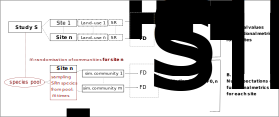
\includegraphics[scale=0.60]{figures/chapter3/chart_FD_calculations}
\caption[Design for calculating functional indices and null expectations for PREDICTS sites]{\textbf{Design for calculating functional indices and null expectations for PREDICTS sites.} \textbf{(A)} Empirical values for the functional diversity indices were obtained for each PREDICTS site, nested within studies. Each site was characterised by its species richness and its land-use. \textbf{(B)} For a given site \textit{n} of richness SR$_{n}$, the community composition was randomised \textit{m} times by drawing SR$_{n}$ species from the study's species pool. Null expectations for the site \textit{n} were then obtained by taking the median value of the indices across simulations.}
\label{FDcalc_chart}
\end{figure}

\subparagraph{Simulation results, and hypotheses as to why simulations may be inadequate.}
Simulation results showed that land-use was having an effect on median simulated values. A decrease in the mean effect was observed for xx and xx, decrease which was significant in some cases, contradicting \textit{expectation 1}. Similarly, a decrease in the slope of the DFR--species richness relationship was observed, contradicting \textit{expectation 2}. I here propose a mechanism that may explain why simulated results differed from my expectations. Simulations were based on the randomisation of the species composition of each site. Species were drawn at random from the species pool, defined as the set of species in each study (equivalent to a `regional' species pool). As such, simulations were sensitive to the composition of the species pool. Nevertheless, the PREDICTS database has an imbalanced design, such that each study do not have sites in all of the land-uses. This may be constricting species pools in some cases. For instance, for a site of land-use `Pasture' belonging to a study where primary vegetation was also sampled, the species pool may be bigger than for a site of land-use `Pasture' where only pasture and plantation forest were sampled. As such, biases in species pool may influence simulation results. Simulation results may capture trends reflecting differences in the size and composition of species pool, which may explain the patterns observed in Figure xx and xx. Figure XX shows Rao's quadratic entropy calculated on the study species pool of each study.

\subparagraph{Simulation approach: conclusion.} The imbalanced design of the PREDICTS database may be causing biases in species pool, which may render simulation approaches difficult to interpret. As such, the simulation approach was not developed further here.

\subsubsection{Dendrogram-based functional richness}
A Gower dissimilarity matrix was first computed from the trait dataset, using the gowdis R function (FD package). This distance matrix contained pairwise distances across all terrestrial vertebrates, based on their trait values. Gower distances allowed to include mixed type variables in the computation. In a second step, this dissimilarity matrix was clustered, to obtain a functional dendrogram, where species presenting similar functional characteristics were closer than more dissimilar species. I used the hclust function, which offers a range of clustering methods. As different clustering methods can have a strong influence on the output dendrogram, I selected the clustering method that best reflected the initial distances in the Gower matrix (correlation coefficient between cophenetic distances obtained from the cluster dendrograms and between the initial dissimilarities in the Gower matrix). The `average' method (unweighted pair group method with arithmetic mean, UPGMA) presented the best correlation coefficient and was as such selected. The resulting cluster dendrogram was a functional dendrogram with 34377 tips, where each tip represented a species. Species position in the tree depended on their functional attributes: species that were functionally more similar were more closely related in the tree.

Finally, functional richness was calculated across all PREDICTS sites. At each site, vertebrate community composition was assessed (species presence/absence), and the functional dendrogram was subsetted according to local community composition. For a site, functional richness was calculated as the sum of the branch length, from root to tip, for the local subset of the functional dendrogram (treedive).


\section{Results}

\subsection{Land-use change constricts the multivariate trait range}
Land-use had a significant effect on volume-based functional richness (Figure \ref{LU_mean_FRic}). For mature and intermediate secondary vegetation, the mean functional richness was similar to that of primary vegetation. For all other more disturbed land-uses, mean functional richness was significantly different from the mean functional richness of primary vegetation, and decreased alongside the land-use gradient. 

\begin{figure}[h!]
\centering
\includegraphics[scale=0.70]{figures/chapter3/FRic/Mean_effect_LU}
\caption[Mean effect of land-use on the volume-based functional richness of vertebrate communities]{\textbf{Mean effect of land-use on the volume-based functional richness of vertebrate communities.} PV: primary vegetation; MSV; mature secondary vegetation; ISV: intermediate secondary vegetation; YSV: young secondary vegetation; PF: plantation forest; CR: cropland; UR: urban. The mean effect corresponds to the estimated fixed effect of a mixed-effect model.}
\label{LU_mean_FRic}
\end{figure}

Because volume-based functional richness is a multivariate analogue of the functional range, Figure \ref{LU_mean_FRic} shows that land-use change significantly impacts the functional composition of local vertebrate communities: species located at the periphery of the functional convex hull are likely to be removed in disturbed land-uses. As such, land-use change significantly impacts the functional composition of local vertebrate communities by constricting the breadth of functions.   

\subsection{Land-use change promotes the functional homogenisation of local vertebrate communities}

\subsubsection{Significant decreases in multivariate trait dispersion}
\begin{figure}[h!]
\centering
\includegraphics[scale=0.70]{figures/chapter3/RaoQ/Mean_effect_FRaoQ}
\caption[Mean effect of land-use on Rao's quadratic entropy in vertebrate communities]{\textbf{Mean effect of land-use on Rao's quadratic entropy in vertebrate communities.} PV: primary vegetation; MSV; mature secondary vegetation; ISV: intermediate secondary vegetation; YSV: young secondary vegetation; PF: plantation forest; CR: cropland; UR: urban. The mean effect corresponds to the estimated fixed effect of a mixed-effect model.}
\label{LU_mean_FRic}
\end{figure}

%% decreases of functional dissimilarities among species: species become more similar

\subsubsection{Functional redundancy increases}
\begin{figure}[h!]
\centering
\includegraphics[scale=0.70]{figures/chapter3/FRedundancy/Mean_effect_LU}
\caption[Mean effect of land-use on the functional redundancy of vertebrate communities]{\textbf{Mean effect of land-use on the functional redundancy of vertebrate communities.} PV: primary vegetation; MSV; mature secondary vegetation; ISV: intermediate secondary vegetation; YSV: young secondary vegetation; PF: plantation forest; CR: cropland; UR: urban. The mean effect corresponds to the estimated fixed effect of a mixed-effect model.}
\label{LU_mean_FRic}
\end{figure}



\section{Discussion}
% sensitivity to trait inclusion
% traits that were not considered that could be important, noably home range, dispersal abilities, or volancy -- traits relating to species abilities to move.